\section{Lab 2: Poisson's equation}

% One can thus implement the different schemes like red-black Gauss-Seidel iteration. This leads to
% a parallel program. However, there are numerous questions or problems that are worth to investigate.
% For instance, is it worth to make more than 1 iteration in each domain between two communication
% steps? The convergence of the algorithm will be slower if measured in the number of iteration steps,
% but if measured in real time it may or may not be advantageous. How much data should one transfer
% in a communication step? Just the data along the border, or maybe more layers at once? What is
% the best way to partition the grid points in to domains? Should these domains be as close to a square
% as possible, horizontal strips or vertical strips? How does the performance scale with problem size, or
% with increasing number of processes?

\subsection{Part 1}
\subsubsection{Step 1}

It is simple to understand that the program was indeed executed twice since two pairs of statements are written to the terminal in comparison to one pair before the modifications. Since we are now running the same program in two different nodes this behavior is expected.  

The result is the following
\begin{lstlisting}
    Number of iterations  : 2355
    Elapsed processortime : 1.350000 s
    Number of iterations  : 2355
    Elapsed processortime : 1.360000 s
\end{lstlisting}

\subsubsection{Step 2}

After adding the global variable and the necessary call to \texttt{MPI\_Comm\_rank} using the predefined communicator \texttt{MPI\_COMM\_WORLD}.
\begin{lstlisting}
    MPI_Comm_rank(MPI_COMM_WORLD, &proc_rank);
\end{lstlisting}

The following is printed to the standard output:
\begin{lstlisting}
    (0)     Elapsed processortime : 1.360000 s
    (0)     Number of iterations  : 2355
    (1)     Elapsed processortime : 1.360000 s
    (1)     Number of iterations  : 2355
\end{lstlisting}

\subsubsection{Step 3}

% After rewriting the timing functions mentioned in the exercise description, the new output is as follows:
% \begin{lstlisting}
%     (0)     Elapsed Wtime        : 1.410156 s ( 97.2% CPU)
%     (0)     Number of iterations : 2355
%     (1)     Elapsed Wtime        : 1.468750 s ( 94.0% CPU)
%     (1)     Number of iterations : 2355
% \end{lstlisting}

\subsubsection{Step 4}

Adjusting the code so each process writes to a separate file does not affect the text displayed, so there is no need to repeat it here. In addition by executing the command

\begin{lstlisting}
    diff output0.dat output1.dat
\end{lstlisting}

I was able to confirm the files are indeed identical.

\subsubsection{Step 5}

On this step, responsible to ensure correct distribution of information originated from an input file, several statements had to be rewritten. Below is a summary of those changes, in particular the parts that were not completely specified in the exercise manual.

To ensure only process 0 opens the file a simple comparison suffices
\begin{lstlisting}
    /* only process 0 may execute this if */
    if (proc_rank == 0)
    { ... }
\end{lstlisting}

To broadcast the data read from the file it is first necessary to explain which fields the \texttt{MPI\_Bcast(void *buffer, int count, MPI\_Datatype datatype, int root, MPI\_Comm comm))} function requires. 

For our situation the \texttt{buffer} pointer should refer to the address of the variable we want to broadcast. The \texttt{count} relates to the number of entries in the buffer. The \texttt{datatype} should describe the type of data the buffer points to, \eg for integers this should be \texttt{MPI\_INT}. The \texttt{root} is the message broadcaster, in our case node 0. Finally we will use the usual predefined communicator for the last argument \texttt{comm}.

Thus the broadcast calls are as follows
\begin{lstlisting}
    /* broadcast the array gridsize in one call */
    MPI_Bcast(&gridsize      , 2, MPI_INT   , 0, MPI_COMM_WORLD);
    /* broadcast precision_goal */
    MPI_Bcast(&precision_goal, 1, MPI_DOUBLE, 0, MPI_COMM_WORLD);
    /* broadcast max_iter */  
    MPI_Bcast(&max_iter      , 1, MPI_INT   , 0, MPI_COMM_WORLD);
(...)
    /* The return value of this scan is broadcast even though it is no input data */
    MPI_Bcast(&s, 1, MPI_INT, 0, MPI_COMM_WORLD);
(...)
    /* broadcast source_x */
    MPI_Bcast(&source_x  , 1, MPI_DOUBLE, 0, MPI_COMM_WORLD);
    /* broadcast source_y */
    MPI_Bcast(&source_y  , 1, MPI_DOUBLE, 0, MPI_COMM_WORLD);
    /* broadcast source_val */
    MPI_Bcast(&source_val, 1, MPI_DOUBLE, 0, MPI_COMM_WORLD);
\end{lstlisting}

\subsubsection{Step 6}

Following the same approach as in the previous section, only the finished version of incomplete code from the manual will be shown in the excerpt.
\begin{lstlisting}
    MPI_Comm_size(MPI_COMM_WORLD, &P);
    (...)
    MPI_Cart_create(MPI_COMM_WORLD, 2, P_grid, wrap_around, reorder, &grid_comm);
    (...)
    /* Rank of process in new communicator */
    MPI_Comm_rank(grid_comm, &proc_rank);
    /* Coordinates of process in new communicator */
    MPI_Cart_coords(grid_comm, proc_rank, 2, proc_coord);
    (...)
    /* rank of processes proc_top and proc_bottom */
    MPI_Cart_shift(grid_comm, Y_DIR, 1, &proc_top, &proc_bottom);
    /* rank of processes proc_left and proc_right */
    MPI_Cart_shift(grid_comm, X_DIR, 1, &proc_left, &proc_right);
\end{lstlisting}

There a couple new function calls on this code whose arguments I will explain next.
As explained in the exercise description MPI uses the \texttt{MPI\_Cart\_*} function calls to arrange tasks in a virtual process grid.

To create one the API calls needs the previous communicator, in our case we were using \texttt{MPI\_COMM\_WORLD}. \texttt{ndims} and \texttt{dims} define the number of dimensions of the grid and the number of processors in each, respectively. For our example these are 2 and \texttt{P\_grid}. Thereafter the periods specifies if the grid is periodic or not per dimension, and finally if the ranking is reordered or not. These are replaced by the self-explanatory variables \texttt{wrap\_around} and \texttt{reorder}. The new communicator is stored in the address of \texttt{comm\_cart}. From now on all pointers to communicators refer to this one.

\begin{lstlisting}
int MPI_Cart_create(MPI_Comm comm_old, int ndims, int *dims, int *periods, int reorder, MPI_Comm *comm_cart)
int MPI_Cart_coords(MPI_Comm comm, int rank, int maxdims, int *coords)
int MPI_Cart_shift(MPI_Comm comm, int direction, int displ, int *source, int *dest)
\end{lstlisting}

To define the coordinates of the process in the new communicator we use \texttt{MPI\_Cart\_coords}. Here the rank is necessarily the processor rank (\texttt{proc\_rank}), the maximum dimensions is 2. The coordinates of each specified process are stored in the \texttt{proc\_coord} array.

Finally the shift operation returns the shifted source and destination ranks. The direction and displacement quantity arguments are self-evident and are replaced in the program by \texttt{X\_DIR} or \texttt{Y\_DIR} and 1 respectively for horizontal and vertical displacements. In accordance to the outputs source and destination are stored in \texttt{proc\_top} and \texttt{proc\_bottom} or \texttt{proc\_left} and \texttt{proc\_right} depending on the direction. 


The text written to the standard output now features the coordinate of each processor.

\begin{lstlisting}
    (0) Number of iterations : 2355
    (0) (x,y)=(0,0)
    (0) Elapsed Wtime:       1.414062 s ( 96.9% CPU)
    (1) Number of iterations : 2355
    (1) (x,y)=(1,0)
    (1) Elapsed Wtime:       1.464844 s ( 95.6% CPU)
\end{lstlisting}

As one can observe since there are two processor, number 0 is allocated the left half of the grid, and processor with rank 1 deals with the right half.

\subsubsection{Step 7}
% After adjusting the \texttt{Setup\_Grid()} function as described the following results were obtained for three different setups. The first has two processors, the second three and the third four. The results can be seen below.

% \begin{lstlisting}
    % (0)   Number of iterations : 1195
    % (0) (x,y)=(0,0)
    % (0) Elapsed Wtime:       0.394531 s ( 86.2% CPU)
    % (1)   Number of iterations : 945
    % (1) (x,y)=(1,0)
    % (1) Elapsed Wtime:       0.347656 s ( 83.4% CPU)

    % (0)   Number of iterations : 1
    % (0) (x,y)=(0,0)
    % (0) Elapsed Wtime:       0.007812 s (  0.0% CPU)
    % (1)   Number of iterations : 695
    % (1) (x,y)=(1,0)
    % (1) Elapsed Wtime:       0.214844 s ( 79.1% CPU)
    % (2)   Number of iterations : 1
    % (2) (x,y)=(2,0)
    % (2) Elapsed Wtime:       0.046875 s (106.7% CPU)

    % (0)   Number of iterations : 791
    % (0) (x,y)=(0,0)
    % (0) Elapsed Wtime:       0.128906 s ( 85.3% CPU)
    % (1)   Number of iterations : 792
    % (1) (x,y)=(0,1)
    % (1) Elapsed Wtime:       0.160156 s ( 99.9% CPU)
    % (2)   Number of iterations : 1
    % (2) (x,y)=(1,0)
    % (2) Elapsed Wtime:       0.058594 s ( 68.3% CPU)
    % (3)   Number of iterations : 791
    % (3) (x,y)=(1,1)
    % (3) Elapsed Wtime:       0.164062 s ( 97.5% CPU)
% \end{lstlisting}

When there are three processors the work can not be evenly split between them. This can be confirmed by inspecting the \texttt{x} and \texttt{y} variables in the \texttt{Setup\_grid function}.

For example for processor 2 (in a 3 processor configuration) it is visible that \texttt{x} is always negative.

\begin{lstlisting}
    (2) x = -30, dim[X_DIR] = 36
    (2) y =  71,  dim[Y_DIR] = 102

    (2) x = -3, dim[X_DIR] = 36
    (2) y = 76, dim[Y_DIR] = 102

    (2) x = -28, dim[X_DIR] = 36
    (2) y =  26, dim[Y_DIR] = 102
\end{lstlisting}


\subsubsection{Step 8}
\subsubsection{Step 9}

After implementing the collective reduction operation the total number of iterations is indeed the same, as confirmed by the program's output.

\begin{lstlisting}
    (0) Number of iterations : 2355
    (0) Elapsed Wtime:       1.507812 s ( 96.2% CPU)
    (1) Number of iterations : 2355
    (1) Elapsed Wtime:       1.496094 s ( 97.6% CPU)
    (2) Number of iterations : 2355
    (2) Elapsed Wtime:       1.507812 s ( 96.8% CPU)
\end{lstlisting}

\subsubsection{Step 10}


\subsection{Part 2}

\subsubsection{2.1}
\subsubsection{2.2}

After changing the code to accommodate for the algorithmic improvement, 5 tests were performed to compare different values for the relaxation parameter $\omega$. The results are summarized in table~\ref{tbl:omega}.
From this data we concluded that 1.93 is the optimal value for the relaxation parameter, accomplishing almost 18 times less iterations than the original with $\omega$ equal to one.

\begin{table}[H]
\centering
\begin{tabular}{cccc}
 \toprule
$\omega$ & \texttt{Wtime}\tablefootnote{This value was computed as the maximum \texttt{Wtime} over the four individual processor times for each $\omega$ value.} (\si{s}) & $n$ & Reduction\\ \midrule
    1.00 &        1.500000 &        2355 &        1.00 \\    
    1.90 &        0.222656 &        220  &        10.7 \\
    1.92 &        0.199219 &        165  &        14.3 \\
\bf 1.93 &    \bf 0.175781 &    \bf 131  &    \bf 18.0 \\
    1.94 &        0.289062 &        142  &        16.6 \\
    1.98 &        0.351562 &        419  &        5.62 \\
\bottomrule
\end{tabular}
\caption{Time, number of iterations obtained and respective iteration reduction for different $\omega$ values. The topology used was \texttt{pt:}441 with a grid size of \texttt{g:}100x100.}
\label{tbl:omega}
\end{table}


\subsubsection{2.3}

The goal of this exercise is to investigate the scaling behavior of the code with a fixed relaxation parameter. To accomplish that analysis several runs were measured with various grid sizes. In addition different \emph{slices} were also tested.

\begin{table}[H]
\centering
\begin{tabular}{*{5}{c}}
 \toprule
          &     & \multicolumn{2}{c}{\texttt{Wtime} (\si{s})} & \\
Grid Size & $n$ & \texttt{pt:}441 & \texttt{pt:}422           & $\Delta$ (\%)\\ \midrule
\multirow{4}{*}{200}
    &    50   &     0.164 &     0.164 &     0.00 \\
    &    100  &     0.226 &     0.246 &     8.62 \\
    &    200  &     0.343 &     0.335 &    -2.27 \\
    &    300  &     0.464 &     0.449 &    -3.36 \\\\
\multirow{4}{*}{400}                                        
    &    100  &     0.437 &     0.460 &     5.36 \\
    &    300  &     1.054 &     1.054 &     0.00 \\
    &    500  &     1.746 &     1.667 &    -4.47 \\
    &    1000 &     3.308 &     3.304 &    -0.12 \\\\
\multirow{4}{*}{800}
    &    100  &     1.414 &     1.445 &     2.21 \\
    &    300  &     3.742 &     3.726 &    -0.42 \\
    &    500  &     5.976 &     5.988 &     0.20 \\
    &    1000 &    11.625 &    11.617 &    -0.07 \\\\
\multirow{4}{*}{2000}
    &    100  &     8.218 &     8.234 &     0.19 \\
    &    300  &    21.351 &    21.328 &    -0.11 \\
    &    500  &    34.933 &    35.492 &     1.60 \\
    &    1000 &    68.304 &    67.824 &    -0.70 \\
\bottomrule
\end{tabular}
\caption{The maximum time for different grid sizes and different \emph{slicing} arrangements. The $\Delta$ column compares the relative difference in performance between the two previous columns. The number of iterations for each run was fixed to enable a more accurate comparison. The 200x200 grid size measurements were performed in different conditions in regards to the iteration count since the program converges after 382 iterations.}
\label{tbl:slices}
\end{table}

The results of the aforementioned experiment are shown in table~\ref{tbl:slices}. As one can obverse the different domain partitions have little impact in the overall performance of the program, even as the grid size increases.


As explained in the exercise manual the (average) time $t$ per iteration $n$ can be parametrized as follows
\begin{equation}
t(n) = \alpha + \beta \cdot n
\label{eq:alphabeta}
\end{equation}

Where $\alpha$ and $\beta$ are arbitrary constants. To determine these constants we will use the least-squares method. The results of applying this technique\tablefootnote{The Google Drive implementation of least-squares, \emph{LINEST} function, was used for this computation. For more information please see \url{https://support.google.com/drive/answer/3094249}.} to the available dataset are shown in table~\ref{tbl:alphabeta}

\begin{table}[H]
\centering
\begin{tabular}{*{5}{c}}
 \toprule
            &    \multicolumn{2}{c}{\texttt{pt:}441} & \multicolumn{2}{c}{\texttt{pt:}422} \\
Grid Size   &    $\alpha$ &    $\beta$                & $\alpha$    & $\beta$ \\ \midrule
200         &    0.105    &    0.001                  & 0.120       & 0.001   \\
400         &    0.116    &    0.003                  & 0.115       & 0.003   \\
800         &    0.310    &    0.011                  & 0.329       & 0.011   \\
2000        &    1.449    &    0.067                  & 1.721       & 0.066   \\
\bottomrule
\end{tabular}
\caption{Using least-squares method we estimated $\alpha$ and $\beta$ as defined in equation~\ref{eq:alphabeta}. The dataset adopted for this computation is present in table~\ref{tbl:slices}.}
\label{tbl:alphabeta}
\end{table}

In order to improve the quality of this an estimation a thorougher study should be performed with more runs. In addition considering other (non-linear) parametrization functions, \eg exponential, may also yield interesting results.

To conclude this question we plotted the estimated functions along with the actual data points to facilitate a visual comparison of the estimation.

% \begin{tikzpicture}
%     \begin{axis}[
%         xlabel=$n$,
%         ylabel=$t$
%         % xmin=0,xmax=300,
%         title=http://cryogenics.nist.gov/,
%         legend style={at={(0.95,0.05)},anchor=south east},
%     ]
%     \addplot[mark=x, color=blue] plot coordinates {
%         (50,  0.164062)
%         (100, 0.226562)
%         (200, 0.343750)
%         (300, 0.464844)
%     };
%     \addlegendentry{441}

%     \addplot[mark=x, color=red] plot coordinates {
%         (50, 0.164062)
%         (100, 0.246094)
%         (200, 0.335938)
%         (300, 0.449219)
%     };
%     \addlegendentry{422}
%     \end{axis}
% \end{tikzpicture}

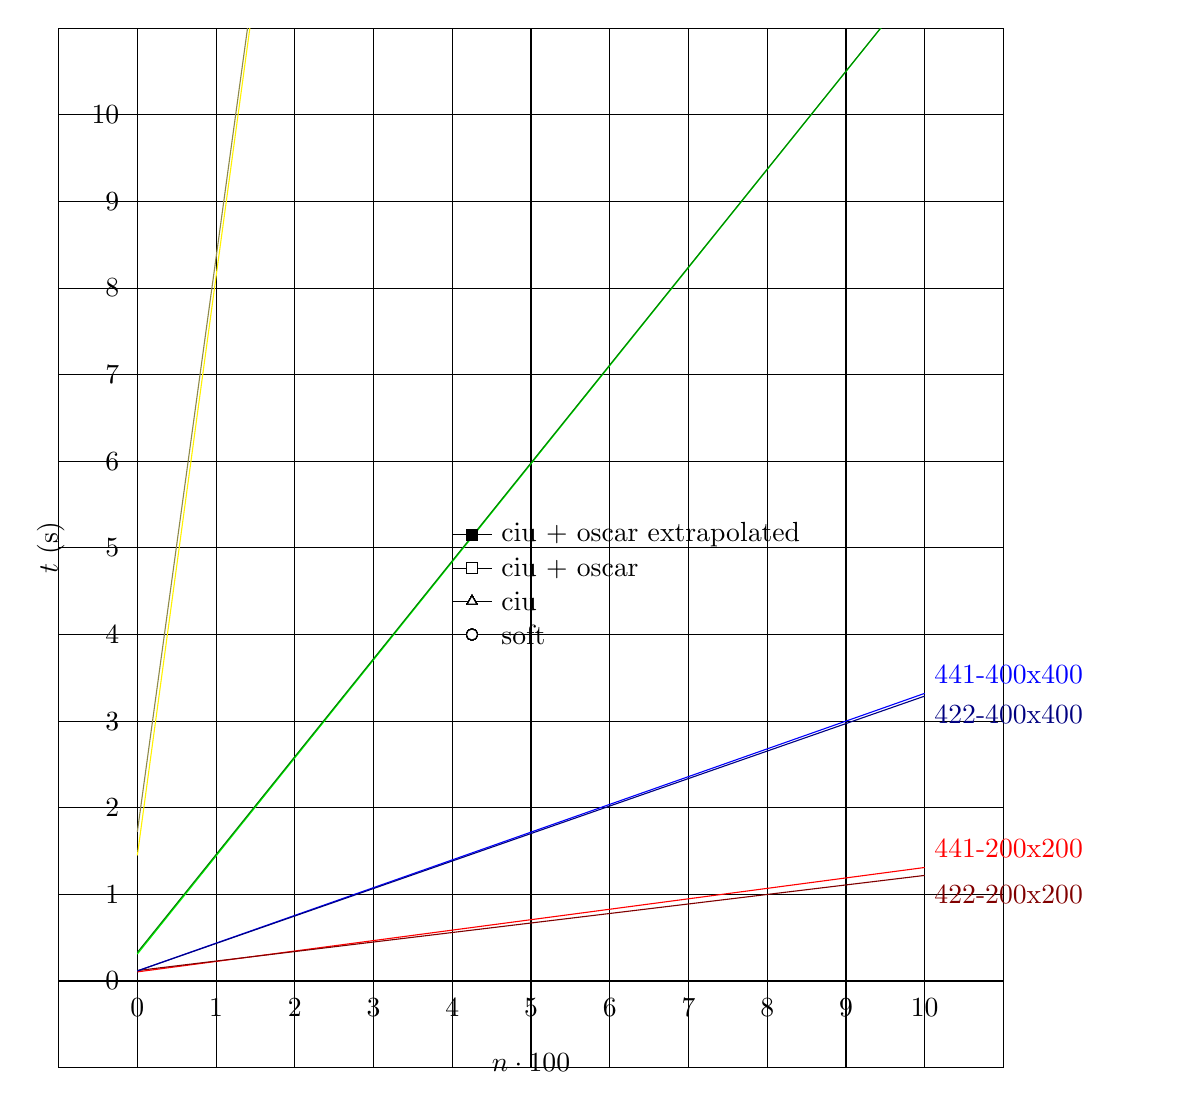
\begin{tikzpicture}[y=1.1cm, x=1.0cm]
    \draw[step=1.0,black,thin] (-1,-1) grid (11,11);
    %axis
    \draw (0,0) -- coordinate (x axis mid) (10,0);
        \draw (0,0) -- coordinate (y axis mid) (0,10);
        %ticks
        \foreach \x in {0,...,10}
            \draw (\x,1pt) -- (\x,-3pt)
            node[anchor=north] {\x};
        \foreach \y in {0,1,...,10}
            \draw (1pt,\y) -- (-3pt,\y) 
                node[anchor=east] {\y}; 
    %labels      
    \node[below=0.8cm] at (x axis mid) {$n \cdot 100$};
    \node[rotate=90, above=0.8cm] at (y axis mid) {$t$ (\si{s})};

    %plots
\begin{scope}
    \clip (-1,-1) rectangle (13,11);

    \draw[color=red]             plot[only marks, mark=*]         file {441-200x200.data};
    \draw[color=red!50!black]    plot[only marks, mark=triangle*] file {422-200x200.data};
    \draw[color=blue]            plot[only marks, mark=*]         file {441-400x400.data};
    \draw[color=blue!50!black]   plot[only marks, mark=triangle*] file {422-400x400.data};
    \draw[color=green]           plot[only marks, mark=*]         file {441-800x800.data};
    \draw[color=green!50!black]  plot[only marks, mark=triangle*] file {422-800x800.data};
    \draw[color=yellow]          plot[only marks, mark=*]         file {441-2000x2000.data};
    \draw[color=yellow!50!black] plot[only marks, mark=triangle*] file {422-2000x2000.data};

    \draw[color=red, domain=0:10]             plot (\x, {0.001198*100*\x+0.105071}) node[above right] {441-200x200};
    \draw[color=red!50!black, domain=0:10]    plot (\x, {0.00110*100*\x+0.12023})   node[below right] {422-200x200};
    \draw[color=blue, domain=0:10]            plot (\x, {0.003200*100*\x+0.116686}) node[above right] {441-400x400};
    \draw[color=blue!50!black, domain=0:10]   plot (\x, {0.00317*100*\x+0.11562})   node[below right] {422-400x400};
    \draw[color=green, domain=0:10]           plot (\x, {0.011324*100*\x+0.310667}) node[above right] {441-800x800};
    \draw[color=green!50!black, domain=0:10]  plot (\x, {0.01130*100*\x+0.32913})   node[below right] {422-800x800};
    \draw[color=yellow, domain=0:10]          plot (\x, {0.066849*100*\x+1.449066}) node[below] {441-2000x2000};
    \draw[color=yellow!50!black, domain=0:10] plot (\x, {0.06631*100*\x+1.72143})   node[below left] {422-2000x2000};
\end{scope}
    
    % legend
    \begin{scope}[shift={(4,4)}] 
    \draw (0,0) -- 
        plot[mark=*, mark options={fill=white}] (0.25,0) -- (0.5,0) 
        node[right]{soft};
    \draw[yshift=\baselineskip] (0,0) -- 
        plot[mark=triangle*, mark options={fill=white}] (0.25,0) -- (0.5,0)
        node[right]{ciu};
    \draw[yshift=2\baselineskip] (0,0) -- 
        plot[mark=square*, mark options={fill=white}] (0.25,0) -- (0.5,0)
        node[right]{ciu + oscar};
    \draw[yshift=3\baselineskip] (0,0) -- 
        plot[mark=square*, mark options={fill=black}] (0.25,0) -- (0.5,0)
        node[right]{ciu + oscar extrapolated};
    \end{scope}
\end{tikzpicture}